
\chapter{Aufgabe D9}
Für die Umsetzung der Warnfunktion durch eine LED, die erst einen Druckabfall-/anstieg signalisiert, wurde eine Statemachine verwendet. Diese besteht aus insgesamt fünf Stati, vier die jeweils 0,8 bzw. 1,6s dauern und die LED aus- bzw. einschalten und dem Off-Status.

\begin{figure}[h!]
	\centering
	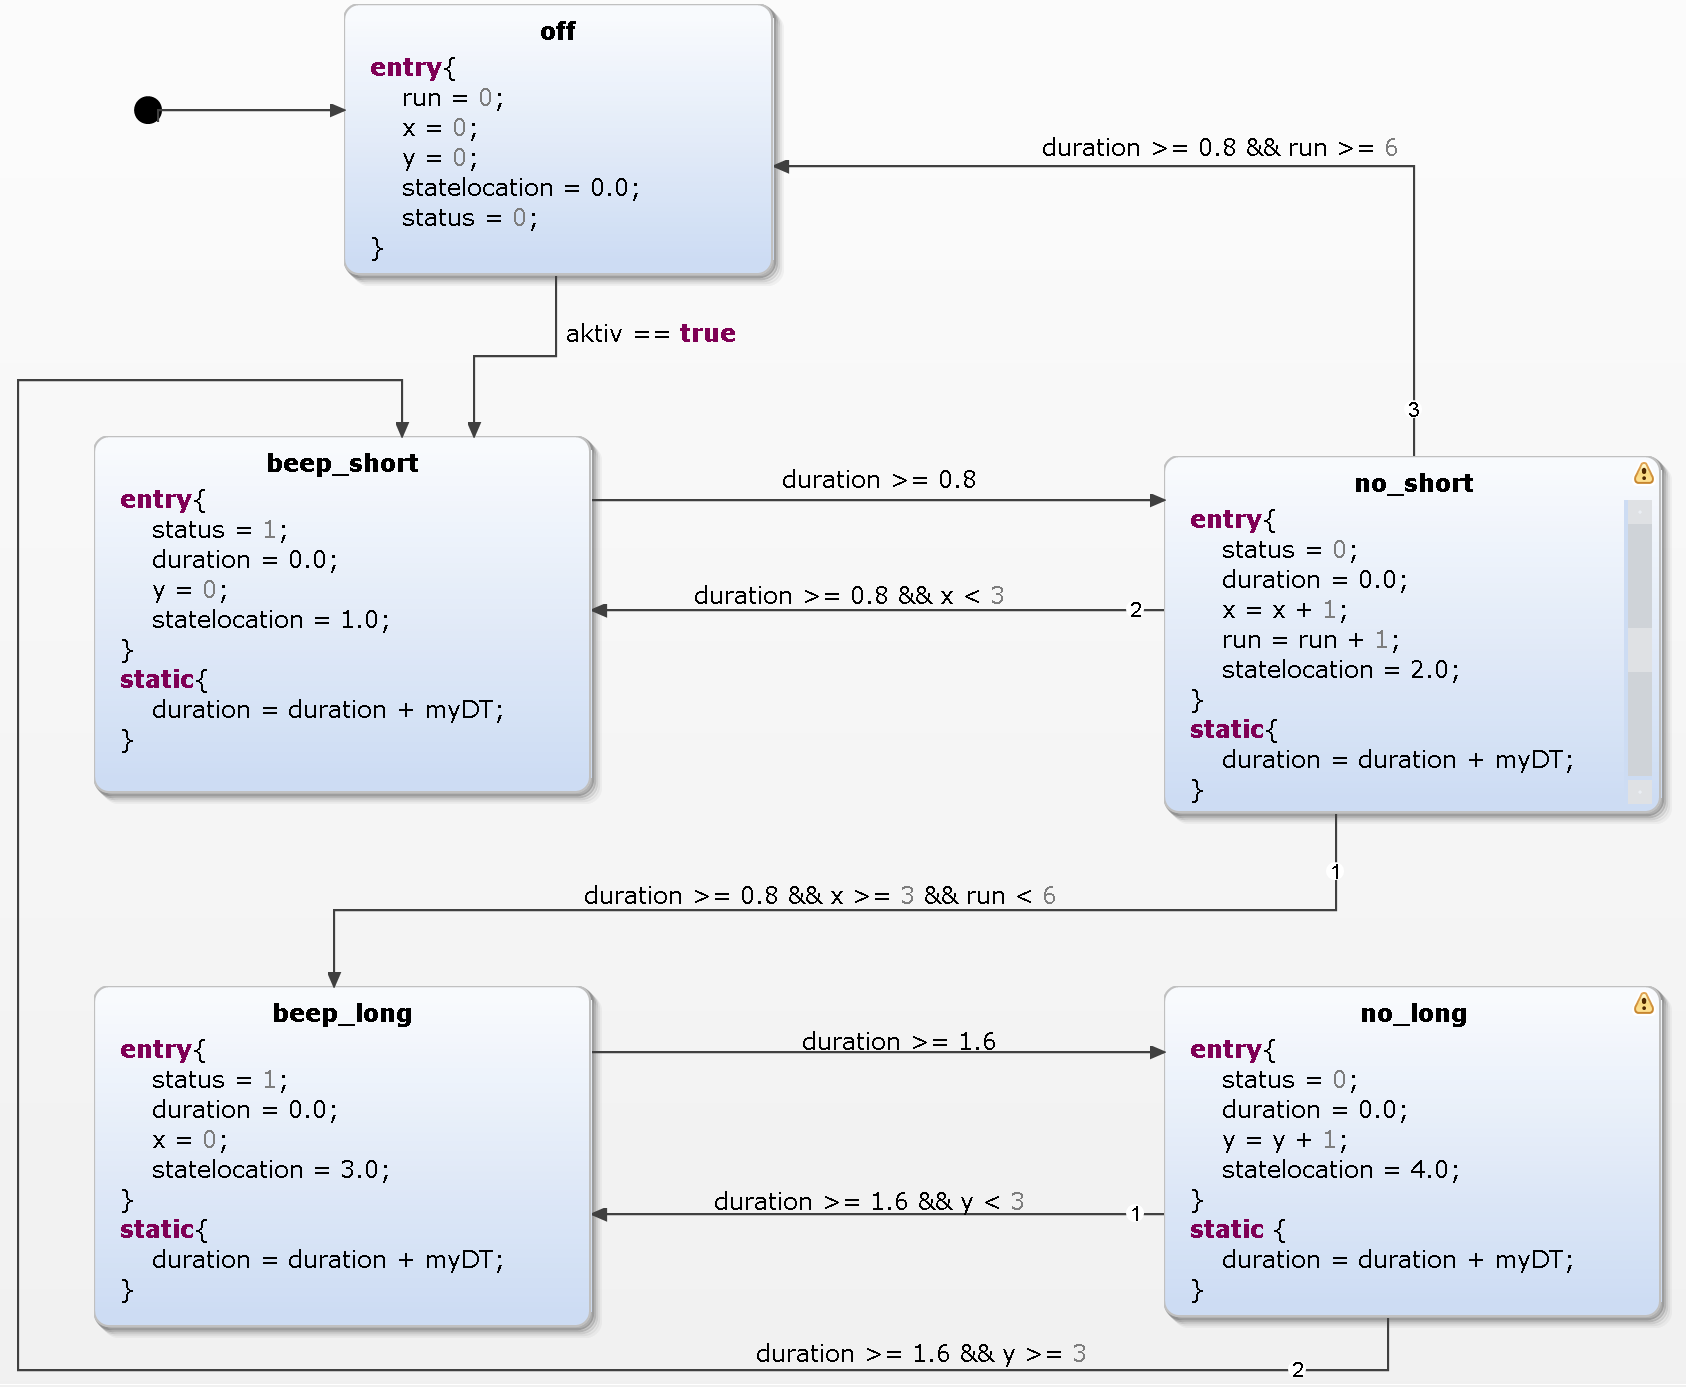
\includegraphics[width=1\linewidth]{../Graphiken/SOS_state.png}
	\caption{SOS Statemachine}
	\label{fig:SOS_state}
\end{figure}